% Nagare Neocognitron pipeline (article Fig. 3). Standalone-compilable: pdflatex fig3-neocognitron.tex
\documentclass[tikz,border=8pt]{standalone}
\usetikzlibrary{positioning,arrows.meta}
\begin{document}
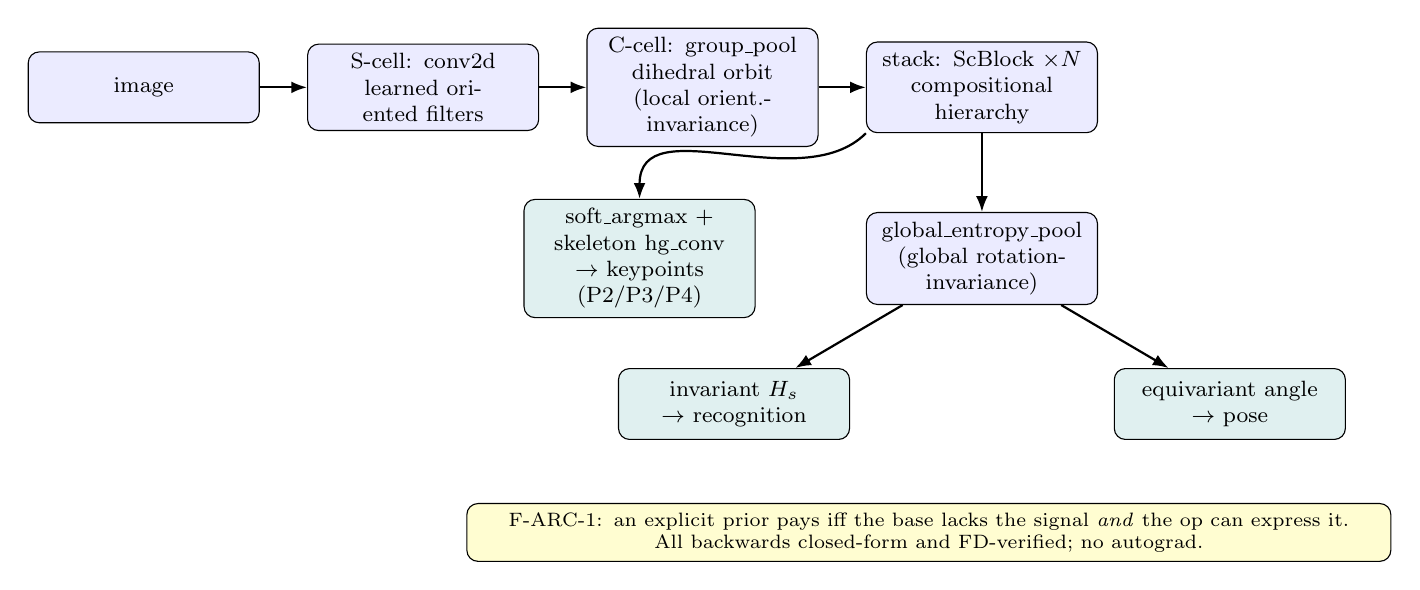
\begin{tikzpicture}[
  font=\footnotesize,
  node distance=6mm,
  b/.style={draw,rounded corners,align=center,minimum height=0.9cm,fill=blue!8,text width=2.7cm},
  h/.style={draw,rounded corners,align=center,minimum height=0.9cm,fill=teal!12,text width=2.7cm},
  note/.style={draw,rounded corners,align=center,fill=yellow!18,text width=11.5cm,font=\scriptsize},
  a/.style={-{Latex[length=2mm]},thick},
]
  \node[b] (img) {image};
  \node[b,right=of img] (s) {S-cell: conv2d\\learned oriented filters};
  \node[b,right=of s]   (c) {C-cell: group\_pool\\dihedral orbit\\(local orient.-invariance)};
  \node[b,right=of c]   (stk){stack: ScBlock $\times N$\\compositional hierarchy};

  \node[b,below=10mm of stk] (ep) {global\_entropy\_pool\\(global rotation-invariance)};
  \node[h,below left=8mm and 2mm of ep] (rec) {invariant $H_s$\\$\rightarrow$ recognition};
  \node[h,below right=8mm and 2mm of ep] (pose){equivariant angle\\$\rightarrow$ pose};

  \node[h,left=14mm of ep] (kp) {soft\_argmax + skeleton hg\_conv\\$\rightarrow$ keypoints (P2/P3/P4)};

  \draw[a] (img)--(s); \draw[a] (s)--(c); \draw[a] (c)--(stk);
  \draw[a] (stk)--(ep);
  \draw[a] (ep)--(rec); \draw[a] (ep)--(pose);
  \draw[a] (stk.south west) to[out=-135,in=90] (kp.north);

  \node[note,below=8mm of rec.south east,xshift=1cm]
    {F-ARC-1: an explicit prior pays iff the base lacks the signal \emph{and} the op can express it.\\
     All backwards closed-form and FD-verified; no autograd.};
\end{tikzpicture}
\end{document}
